\documentclass[t]{beamer}
\usepackage{CJKutf8}
\usepackage{amsfonts}
    \usepackage{amsmath}
    \usepackage{amssymb}
    \usepackage{amsthm}
    \usepackage{enumerate}
    \usepackage{graphicx}
    \usepackage{layout}
    \usepackage{mathrsfs}
    \usepackage{fancyhdr}
    \usepackage{subfigure}
    \usepackage{tcolorbox}
    \usepackage{tikz-cd}
    \usepackage{color}
    \usepackage{pifont}
    \usepackage{verbatim}
    \usepackage{mathtools}
    \usepackage{float}
    \usepackage{bm}
    \usetheme{AnnArbor}
% \usetheme{Antibes}
\usecolortheme{beaver}
\usepackage{listings}

% 设置JSON样式
\lstdefinestyle{json}{
    basicstyle=\tiny\ttfamily,
    columns=fullflexible,
    showstringspaces=false,
    commentstyle=\color{gray},
    keywordstyle=\color{blue},
    stringstyle=\color{red},
    breaklines=true,
    frame=single,
    captionpos=b,
    aboveskip=10pt,
    belowskip=10pt
}

\lstset{
    language=Python, % 设置代码块语言为Python
    breaklines=true, % 自动换行
    basicstyle=\small\ttfamily, % 设置基本字体样式
    keywordstyle=\bfseries\color{blue}, % 设置关键字样式
    commentstyle=\itshape\color{gray}, % 设置注释样式
    showstringspaces=false, % 不显示字符串中的空格
    frame=single, % 设置代码块边框样式
    numbers=left, % 行号显示在左侧
    numberstyle=\tiny\color{gray}, % 设置行号样式
    stepnumber=1, % 设置行号间隔
    tabsize=4 % 设置制表符宽度
}


% 设置shell样式
\lstdefinestyle{shell}{
    language=bash,
    basicstyle=\tiny\ttfamily,
    columns=fullflexible,
    showstringspaces=false,
    commentstyle=\color{gray},
    keywordstyle=\color{blue},
    stringstyle=\color{red},
    breaklines=true,
    frame=single,
    captionpos=b,
    aboveskip=10pt,
    belowskip=10pt
}

% 添加网址的命令
\usepackage{hyperref}
% 这是一个带链接文本的示例:\href{https://www.example.com}{点击这里访问网站}
% 普通的示例:\url{https://www.example.com}
% 表格
\usepackage{booktabs}
\usepackage{multirow}

% \setbeamertemplate{navigation symbols}{}

\usepackage{textpos}

\newcommand{\dif}{\mathrm{d}}
\newtheorem{thm}{{定理}}

% some common command
\newcommand{\mm}[1]{$ #1$\newline}
% \newcommand{\tuichu}{\Rightarrow}
% \newcommand{\li}[1]{\newline#1}



\newcommand{\analysis}[2]{\forall \mathcal{E}{#1},\exists \delta {#2},s.t.}
\newcommand{\denyanalysis}[2]{\exists \mathcal{E}{#1},\forall \delta {#2},s.t.}
\newcommand{\yield}{\Rightarrow }
\newcommand{\jj}{\newline}
\newcommand{\ff}[1]{$ #1$}   % math environment + newline
\newcommand{\fgn}[1]{\begin{equation}#1\end{equation}  }
\newcommand{\fg}[1]{$$ #1$$}   % math environment + newline 
\newcommand{\pf}{$proof.$\newline}
\newcommand{\ee}{\newline\ff{\Box}\newline}
\newcommand{\fenshi}[2]{\ff{\frac{#1}{#2}}}
\newcommand{\shenlue}{\vdots\jj}
\newcommand{\abs}[1]{{\left \lvert #1 \right\rvert}}
\newcommand{\loge}[1]{In ({#1})}
\newcommand{\logical}[2]{log_{#2}^{#1}}
\newcommand{\summary}[3]{$\sum_{{#1}={#2}}^{#3}  $}
\newcommand{\denjia}[2]{{#1}\Leftrightarrow {#2}}
\newcommand{\jihe}[3]{ {#1}  = \{ {#2} \mid {#3} \} }
\newcommand{\ve}[2]{\left\langle {#1},{#2}\right \rangle}
\newcommand{\dakuohao}[2]{\begin{array}{rcl}{#1}\end{array} \} \Rightarrow{#2}}
\newcommand{\sxb}[3]{#1^{#2}_{#3}}
\newcommand{\sss}[2]{#1^{#2}}
\newcommand{\xxx}[2]{#1_{#2}}
\newcommand{\bri}[1]{\uppercase\expandafter{\romannumeral#1}}
\newcommand{\ri}[1]{\romannumeral#1} 
\newcommand{\polynomial}[8]{#1_{#2}#6^{#7}+#1_{#3}#6^{#8}+...+#1_{#4}#6+#1_{#5} }
\newcommand{\newd}[4]{f[{#1}_{#2},{#4},{#1}_{#3}]}
\newcommand{\lb}[2]{\begin{align*}\begin{split}{#1}\{ {#2}\end{split}\end{align*}}
\newcommand{\tab}[1]{\begin{array}{ll} {#1}\end{array}}


% 向量乘积
\newcommand{\avg}[1]{\left\langle #1 \right\rangle}
% 偏微分方程
\newcommand{\difFrac}[2]{\frac{\dif #1}{\dif #2}}
\newcommand{\pdfrac}[2]{\frac{\partial{#1}}{\partial{#2}}}
% 不同章节
\newcommand{\one}[1]{\section{#1}}
\newcommand{\two}[1]{\subsection{#1}}
\newcommand{\three}[1]{\subsubsection{#1}}
\newcommand{\aone}[1]{\section*{#1}}
\newcommand{\atwo}[1]{\subsection*{#1}}
\newcommand{\athree}[1]{\subsubsection*{#1}}
% 大括号,左右都有
\newcommand{\lbra}[1]{\left\{  {\begin{matrix} #1 \end{matrix}}\right. } 
% 样式 括号前缀 + 括号 
\newcommand{\lbras}[2]{{#1}\left\{ {  {\begin{matrix} #2 \end{matrix}}}\right. } 
\newcommand{\rbra}[1]{ \left.  {\begin{matrix} #1 \end{matrix}} \right\}  } 
% 模长
\newcommand{\distance}[1]{\parallel #1\parallel }
% 等价
\newcommand{\equ}{\Longleftrightarrow }
% 共轭
\newcommand{\cja}[1]{\overline{#1}}
% 两个矩阵,上面是 方框[] 下面是线条| 中间是 无
\newcommand{\mtx}[1]{\begin{matrix}#1\end{matrix} }
\newcommand{\bmtx}[1]{\begin{bmatrix}#1\end{bmatrix} }
\newcommand{\vmtx}[1]{\begin{vmatrix}#1\end{vmatrix} }
% \newcommand{\table}[1]{\begin{array}[lr]{ccc} #1 \end{array}}

%输入普通字符
\newcommand{\ww}[1]{\text{#1}}

% 所有内容 直接头文件搞定
\newcommand{\everything}[1]{\begin{document}\begin{CJK*}{UTF8}{gkai}#1\end{CJK*}\end{document}}


% 存放代码(失败了)
\newcommand{\cccode}[1]{\begin{lstlisting}#1\end{lstlisting}}

% 改变特定行序列
\newcommand{\ttt}{\subsection{}}

% 嵌套序号
\newcommand{\eee}[1]{\begin{enumerate}#1\end{enumerate}}


% 模板里面的一些宏
\newcommand{\pdfFrac}[2]{\frac{\partial #1}{\partial #2}}
\newcommand{\OFL}{\mathrm{OFL}}
\newcommand{\UFL}{\mathrm{UFL}}
\newcommand{\fl}{\mathrm{fl}}
\newcommand{\op}{\odot}
\newcommand{\Eabs}{E_{\mathrm{abs}}}
\newcommand{\Erel}{E_{\mathrm{rel}}}
% 变化颜色
\newcommand{\red}{\textcolor{red}}
\newcommand{\blue}{\textcolor{blue}}



% 流程图需要用到的宏包
\usepackage{palatino}
\usepackage{tikz}
\usetikzlibrary{shapes.geometric, arrows}
\tikzstyle{startstop} = [rectangle, rounded corners, minimum width = 2cm, minimum height=1cm,text centered, draw = black, fill = red!40]
\tikzstyle{io} = [trapezium, trapezium left angle=70, trapezium right angle=110, minimum width=2cm, minimum height=1cm, text centered, draw=black, fill = blue!40]
\tikzstyle{process} = [rectangle, minimum width=3cm, minimum height=1cm, text centered, draw=black, fill = yellow!50]
\tikzstyle{decision} = [diamond, aspect = 3, text centered, draw=black, fill = green!30]
% 箭头形式
\tikzstyle{arrow} = [->,>=stealth]
% 4个非常重要 的新命令
\newcommand{\start}[2]{    \node (start) [startstop]{#1};\node (in1) [io, below of = start]{#2};\lin{start}{in1}{}}
\newcommand{\stopp}[3]{\node (out1) [io, below of= #1]{#2};\node (stop) [startstop, below of=out1]{#3};\lin{out1}{stop}{} }
\newcommand{\pro}[6]{    \node (#3) [process, #2 of=#1,xshift=#4 cm]{#5};}
\newpage
\newcommand{\lin}[3]{\draw [arrow] (#1) --node [above] {#3} (#2);}


\begin{document}
\begin{CJK*}{UTF8}{gkai}
% 一般第一页显示PPT标题以及作者信息

% \BackgroundPic{./Screenshot from 2022-04-20 16-31-08.png}

% 增加学校 前面
\addtobeamertemplate{title page}{}{
	\begin{tikzpicture}[remember picture,overlay]
		% \node[yshift=85pt,xshift=50pt]{\includegraphics[height=2cm]{Screenshot from 2022-04-20 16-51-21.png}};
\end{tikzpicture}
}


	% \title{时间序列数据集}
	\title{组会汇报}
	\subtitle {} %不需要
	\author{
		陈钶杰\, \\
		专业:计算数学\,
	} % 显示作者
	% \institute {学院:数学科学学院} % 设置学院机构	
	\date{\today}  % 显示日期
\titlepage

% 设置目录
\begin{frame}{目录}
\frametitle{目录}	
\tableofcontents  % 显示目录
\end{frame} 


\section{论文:PromptCast时间序列预测}



% \subsection{文献1}
% \begin{frame}
%     \frametitle{chatglm2的优势}
%     \begin{itemize}
%         \item 更加强大的性能:效果变得更好
%         \item 更长的上下文,但是chatglm2对于单轮超长文档的理解能力有限,我们会在后续迭代升级中着重优化。
%         \item 更加高效的推理:推理速度更快
%     \end{itemize}
% \end{frame}

% \subsection{文献2}
% \begin{frame}
%     \frametitle{1.3B小模型逆袭大模型的秘密}
%     \begin{itemize}
%         \item 高质量数据来源及其重要性:
%         \item 一般一个6B的语言模型指的是训练这个语言模型用到了6B的tokens,一般微调是远小于这个值的,比如几百万,几千万。
%         \item phi这个语言模型用了7B的tokens就训练出了很好的结果。
%     \end{itemize}
% \end{frame}

% \subsection{文章重点汇总}

% \begin{frame}
%     \frametitle{PromptCast时间序列预测方法的结果}
%     \begin{itemize}
%         \item 摘要:该论文提出了一种名为PromptCast的时间序列预测的新方法,它将数字输入和输出转换为提示,并以逐句的方式构造预测任务。作者还提供了一个大规模数据集(PISA),以支持和促进这项任务的研究。
%         % \item 本文的贡献如下:
%         % \eee{
%         %     \item 本文介绍了一项名为基于提示的时间序列预测(PromptCast)的新任务,该任务从基于语言的角度进行一般的时间序列预测,无需对模型架构进行任何修改。
%         %     \item 作者介绍了第一个大规模数据集PISA(基于提示的时间序列预测),该数据集是为基于即时的时间序列预测任务量身定制的,它将支持PromptCast任务的研究并刺激时间序列分析领域的相关研究。
%         %     \item 本文开发了一种基准,其中报告了多种方法的预测性能,包括基于数值的预测方法和语言生成模型。事实证明,拟议的带有语言生成模型的PromptCast是一个很有前途的研究方向,与传统的基于数值的预测相比,它在零点设置下的概括能力要好得多。
%         % }
%         % \item 本文的导言讨论了越来越多地使用深度学习框架进行时间序列预测的情况,包括基于LSTM、TCN和Transformer的模型。作者还注意到自然语言处理领域大规模预训练模型的增长,并提出了一个问题,即这些模型是否可以适应时间序列预测。本文提出了一种名为PromptCast的时间序列预测的新方法,该方法将数字输入和输出转换为提示,并以逐句的方式构造预测任务。作者还引入了大规模数据集(PISA),以支持和促进这项任务的研究。
%         % \item 该论文提出了一种名为PromptCast的时间序列预测的新方法,它将数字输入和输出转换为提示,并以逐句的方式构造预测任务。作者还引入了大规模数据集(PISA),以支持和促进这项任务的研究。该论文评估了PISA数据集上不同的最先进的基于数值的预测方法和语言生成模型。具有各种预测设置的基准结果表明,拟议的带有语言生成模型的PromptCast是一个很有前途的研究方向。
%         % \item 本文介绍了拟议的PromptCast时间序列预测方法的结果,该方法使用语言生成模型来生成预测的未来描述。作者评估了PISA数据集中三种不同语言模型的性能,并将其与三种天真的预测方法作为基线进行了比较。结果表明,所有三种语言模型都可以生成合理的预测未来描述,缺失率几乎为零。此外,与传统的基于数值的预测相比,PromptCast在零点设置下的概括能力要好得多。总体而言,结果表明,具有语言生成模型的PromptCast是时间序列预测的有前途的研究方向。
%         % \item 该论文提出了一项名为PromptCast的新任务,该任务利用语言模型以语言生成方式预测时间序列。作者构建了第一个数据集PISA,以研究基于即时的预测并在已发布的数据集上建立基准。实验结果表明,在 PromptCast 设置中使用语言模型可以获得良好的预测性能和概括能力。作者得出的结论是,具有语言生成模型的PromptCast是时间序列预测的一个有前途的研究方向。
%         \item 模型框架:\\
%         % 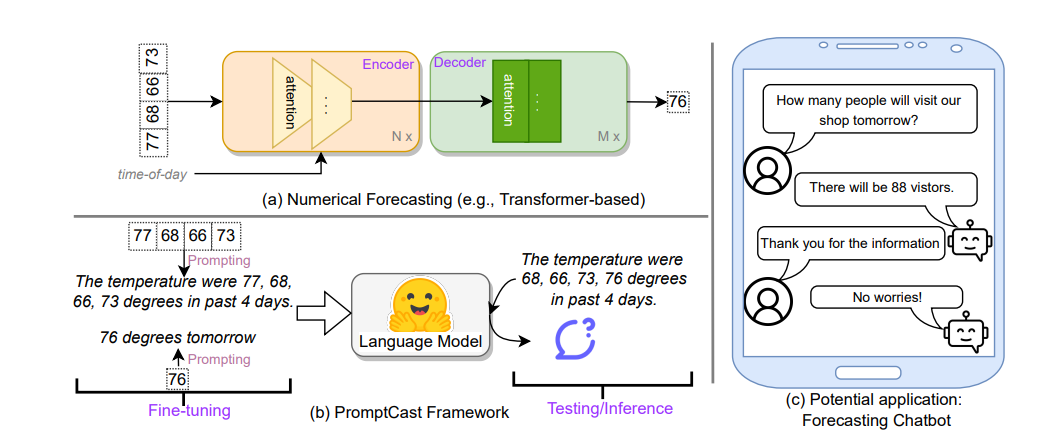
\includegraphics[scale=0.5]{png/PromptCast.png}
%         稍微解释一下这个框架?
%         \item 如何把序列变成自然语言?
%         % 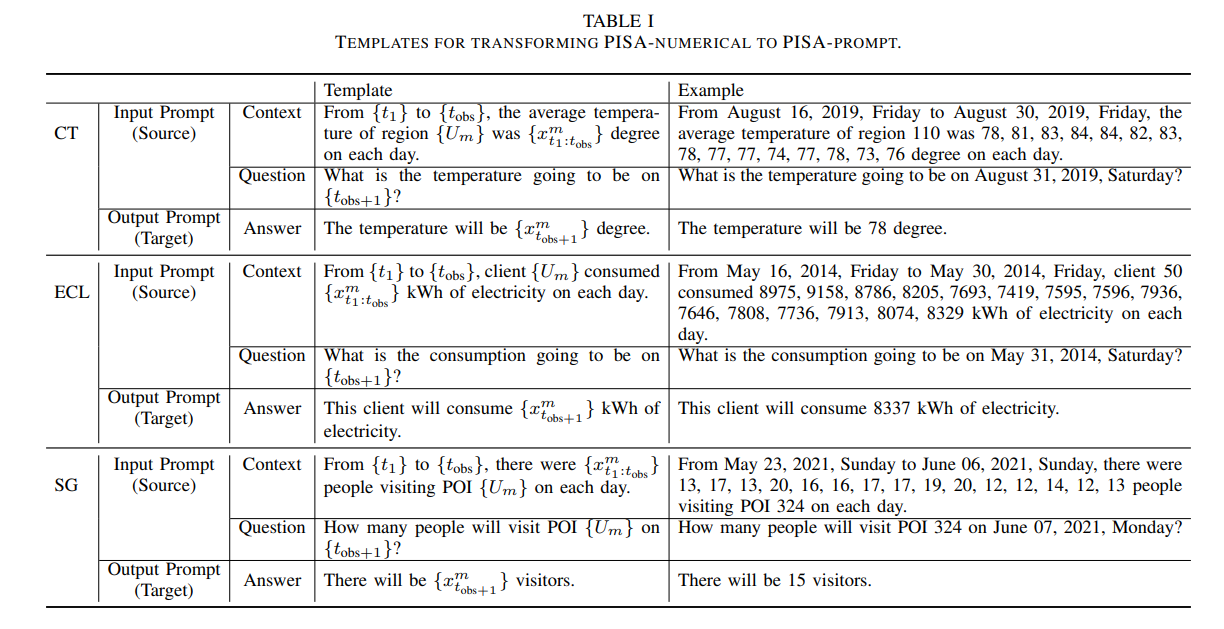
\includegraphics[scale=0.5]{png/prompt_table.png}
%         \item 他的input里面主要有历史的时间序列以及表示要预测的时间序列节点的话语。
%         \item 引入了一个评估指标:缺失率,定义为\ff{
%             \frac{(n_{test})-n_{decoded}}{n_{test}} \times 100\%
%         }其中这个测试是指所有测试集合中的准确率,就是相当于我的精确度,这边使用了准确率。
%         \item 他还引入了其他的评估指标:他的评估指标就是训练运行5次以后把结果取个平均,来避免某次实验的偶然性。
%         \item 一共使用10个语言模型和10个现有的方法进行对比结果
%         \item 他的模型是使用fine-tuning
%         \item 使用预训练模型的权重会让结果变得更加好?
%         \item 评估时间序列的方法:一共三个子集,然后通过训练了其中两个子集再去验证第三个子集,来考虑zero shot的性能。最后明显发现语言模型的性能是要远大于时间序列模型的。
%         \item (1)包括适当的上下文(即使这些上下文提示中不引入额外的数据,例如基本提示)是有益的; \\
%         (2)辅助信息是重要的提示中的组件以获得更好的预测性能。
%         \item 他也做了根据几个序列预测后面几个序列的实验,并且有一个表格完整的表示了出来,看了看他的效果。
%         \item 不同的提示的形式,其中提示C的性能是更加的好,所以我可以尝试去做提示C这种方式!!不好的解释是当前的提示AB不能把不同特征之间的关系描述出来。
%         % 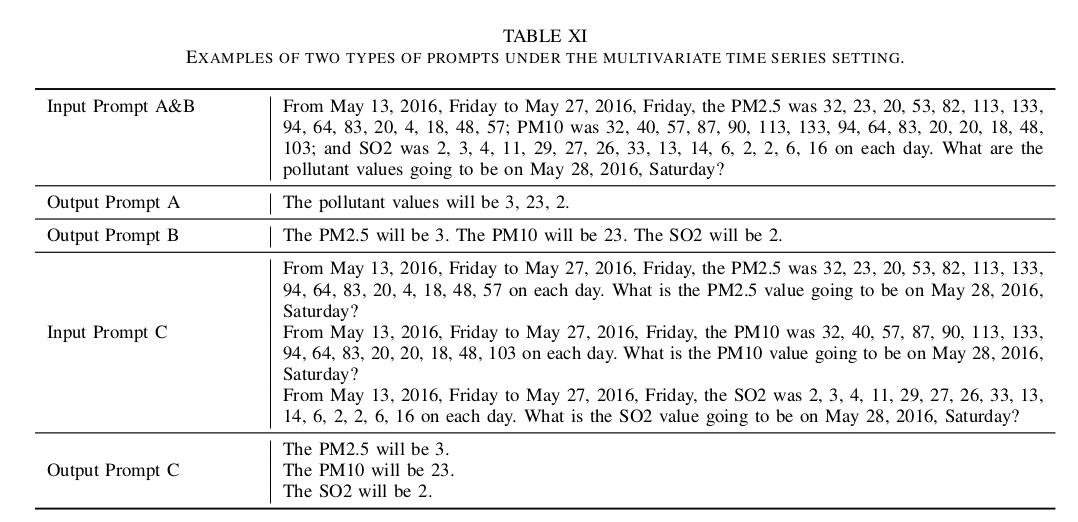
\includegraphics[scale=0.5]{png/prompt_express.png}
%         \item 学习不同时间特征之间的内部相关性,然后开发提示来表示学到的相关性。(一个未来的工作方向)
%         \item 为什么时间序列能够进行预测呢,
%         \item 这个热力图特别有意思,感觉把这个内核都给他挖掘出来了!!??
%         这边这个热力图太秀了,直接将这个时间序列预测的性能挖掘出来了。这个我也可以去挖掘一下出来,感觉太强大了,都不知道是怎么做到的。我只有一种感觉
%         % 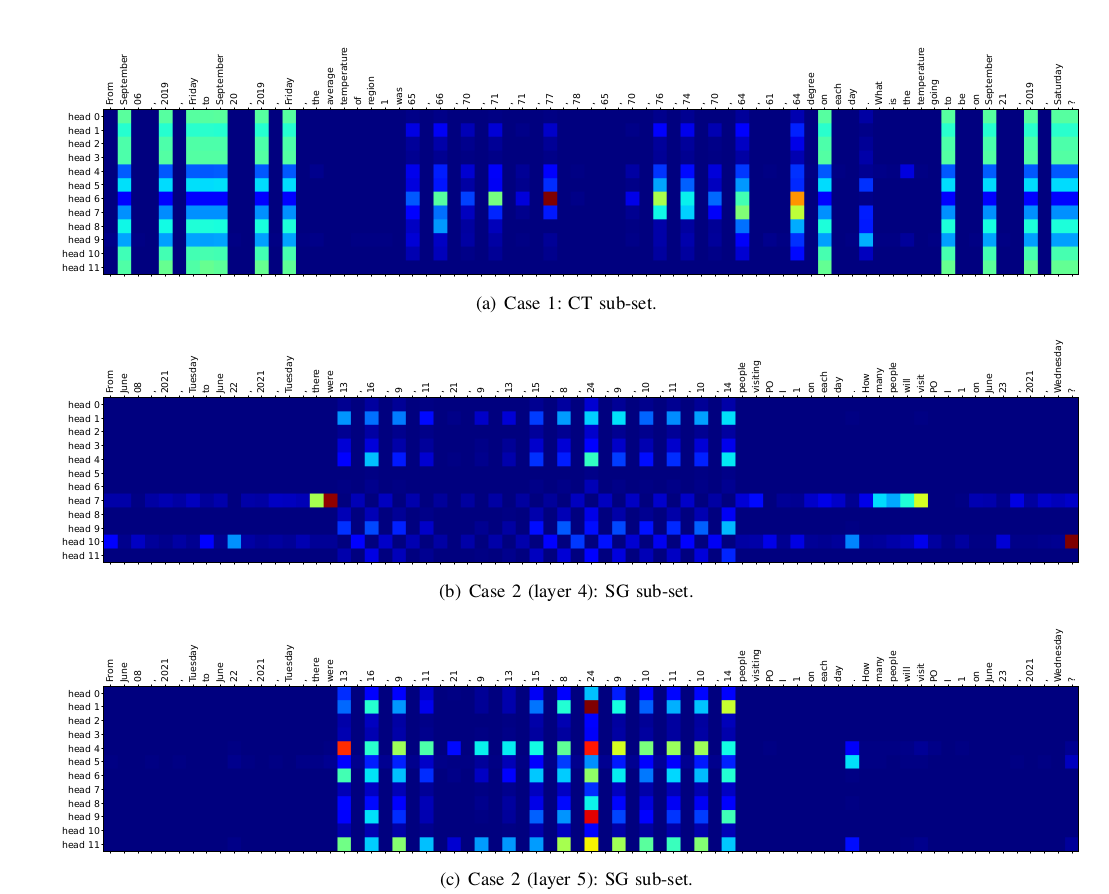
\includegraphics[scale=0.5]{png/prompt_attention.png}
%     \end{itemize}
% \end{frame}


\subsection{文章中和当前工作相似的内容}
\begin{frame}
    \frametitle{input,output形式}
    \begin{itemize}
        \item 该文章中的输入和输出形式和我们的结构基本相同,但他的微调方式是Fine-tuning。\\
        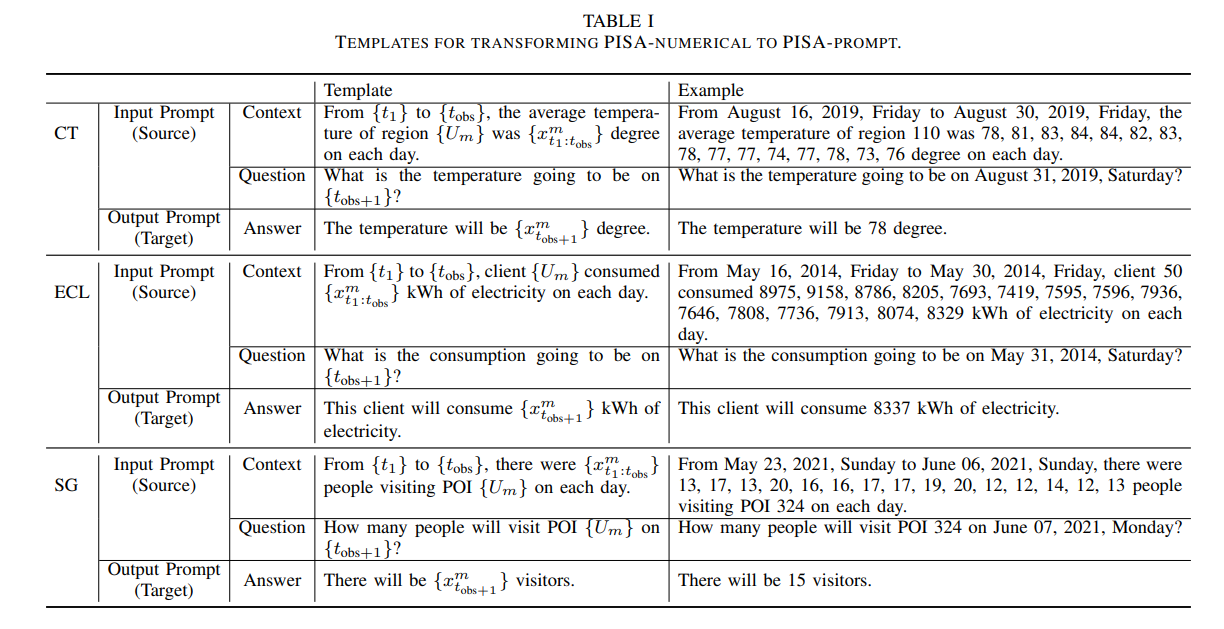
\includegraphics[scale=0.25]{png/prompt_table.png}
    \end{itemize}            
\end{frame}

\begin{frame}
    \frametitle{评估指标}
    \begin{itemize}
        \item 引入了一个评估指标:缺失率,定义为\fg{
            \frac{(n_{test}-n_{decoded})}{n_{test}} \times 100\%
        }
        这个\ff{n_{test}}和\ff{n_{decoded}}分别表示测试的数量和测试集中正确解码的数量。\\
        我在测试的时候,使用的精确度类比这个就是\ff{\frac{n_{decoded}}{n_{test}} \times 100\%}
        \item 文章使用了RMAE,MSE的评估指标。但是文章中进行了五次不同的随机种子运行,并报告了平均性能和标准差。这样做是为了考虑到深度学习方法在不同的随机初始化下可能产生不同的结果。通过进行多次运行并计算平均性能和标准差,可以提供更全面和可靠的评估。
        % 平均性能反映了方法的总体表现水平,而标准差则表示了结果之间的变异程度。
    \end{itemize}
\end{frame}

\subsection{文章中得到的一些启发}
\begin{frame}
    \frametitle{文章的重点实验}
    \begin{itemize}
        \item 他将10个语言模型和10个时间序列模型进行比对,但是语言模型是直接接受三组数据的训练,而时间序列模型是对每组数据进行相应的训练,最终得到了对比的结果。
        \item 测试这些模型的泛化能力:一共三组数据,用其中两组数据对模型进行训练,剩下的一组数据作为测试集合,来测试模型的精确度。最后发现语言模型在完成未见过的任务上要优于其他时间序列模型。
        \item 根据预测长度的对比实验,比如根据前面7天的数据预测后面1天,4天,7天的结果。根据文章的结果可得预测的长度越长,误差就越大,相同的预测长度下,历史数据越多,误差越小。
    \end{itemize}
\end{frame}

\begin{frame}
    \frametitle{文章的重点实验}
    \begin{itemize}
        \item 对于同一个问题,使用不同的提示方式,进行微调,结果也不同。其中提示C的性能更好,可能相比提示C,提示AB中没能把不同特征之间的关系描述出来。因此我之后可以尽可能使用鲜明对比的提示方式。
        
        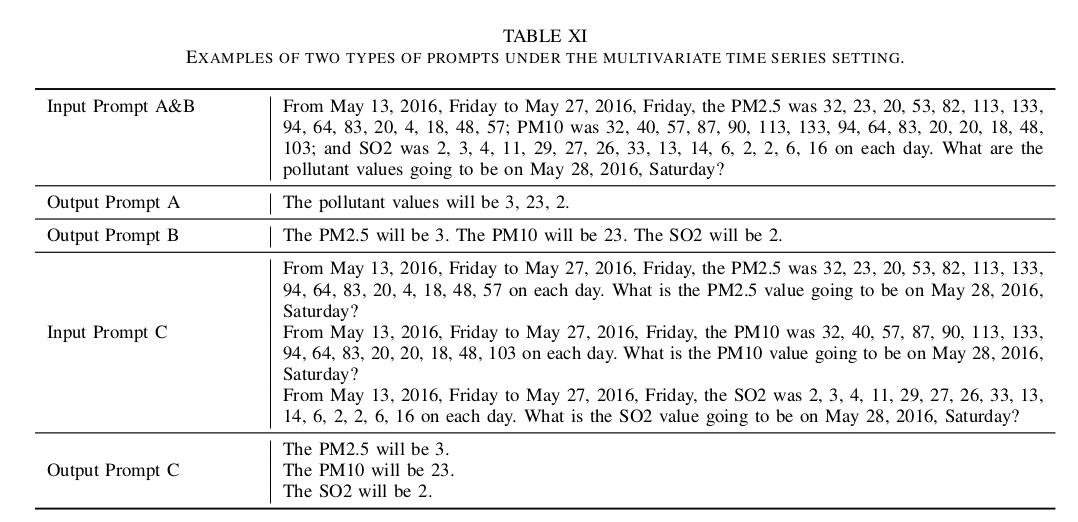
\includegraphics[scale=0.3]{png/prompt_express.png}
    \end{itemize}
\end{frame}

\begin{frame}
    \frametitle{文章的重点实验}
    \begin{itemize}
        \item 探索语言模型可以进行时间序列预测的原因?\\
        通过使用热力图,将提示中的每一个单词的重要性都展示出来了,可以看到越到后面几层,提示中的历史数据就变成最重要的信息了,这不仅说明了这个提示序列的重要性,还说明了这个语言模型确实用到了历史序列的信息,因此能够进行时间序列的预测。
        
        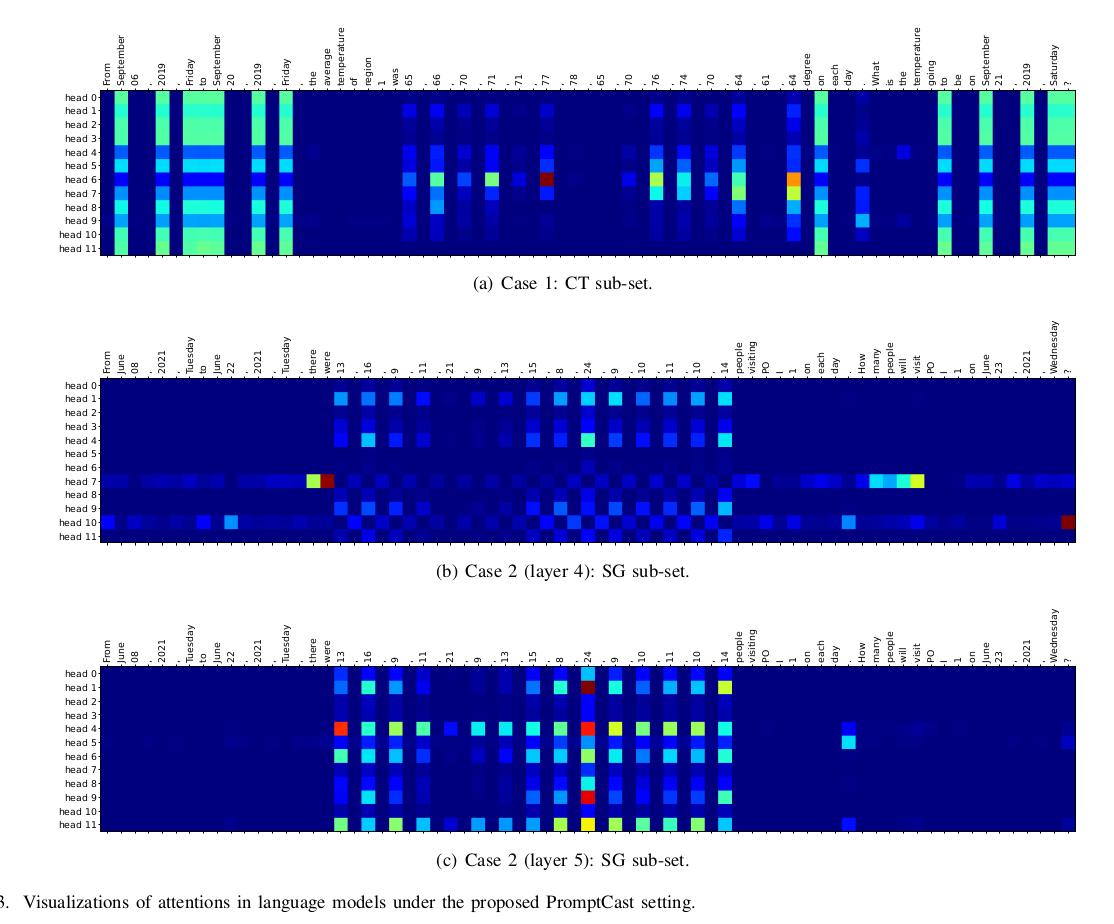
\includegraphics[scale=0.15]{png/prompt_hot.png}
    \end{itemize}
\end{frame}

% \subsection{}
\begin{frame}
    \frametitle{后续相关任务}
    \begin{itemize}
        \item 需要做一个多模型比对实验。
        \item 选择合适的提示方式,参考文章中使用更加能够描述不同特征的提示,并且关于时间的提示只是给定了开始和结尾,可以省略大量的信息。
        \item 在评估RMAE和MSE指标的时候需要进行多次随机种子实验来保证测试的可靠性。
        % \item 模型泛化实验的例子,可以类似的进行。
        \item 可以像文章中使用热力图的方式,将语言模型能够进行预测的内部原因挖掘出来。
    \end{itemize}
\end{frame}



% \subsection{论文2}
% \begin{frame}
%     \frametitle{MEGABYTE的新方法}
%     \begin{itemize}
%         \item 摘要:该论文提出了一种名为MEGABYTE的新方法,用于对超过一百万字节的长序列进行建模。它使用多尺度解码器架构,将序列分成补丁,并在补丁中使用局部子模型,在补丁之间使用全局模型,从而实现次二次自我注意力,提高解码过程中的并行性。
%         \item 本文的贡献如下:
%         \eee{
%             \item 引入 MEGABYTE,这是一种使用多尺度解码器架构对长字节序列进行建模的新方法,该架构将序列分成补丁,在补丁中使用本地子模型,在补丁之间使用全局模型。
%             \item 对 MEGABYTE 和强基线进行了广泛的实验,表明 MEGABYTE 允许字节级模型在长上下文语言建模中与子词模型竞争,在 ImageNet 上实现最先进的密度估计困惑,并允许从原始音频文件进行音频建模。
%             \item 观察到,对于许多任务,大多数字节预测相对容易,这意味着没有必要按字节计算大型网络,并且可以使用小得多的模型进行补丁内建模。
%         }
%         \item introduction:该论文的介绍突显了音乐、图像或视频文件等各个领域中数百万字节的序列无处不在。但是,大型变压器解码器通常只使用数千个上下文令牌,这限制了可以应用它们的任务集。本文介绍了 MEGABYTE,这是一种使用多尺度解码器架构对长字节序列进行建模的新方法,该架构将序列分成补丁,在补丁中使用局部子模型,在补丁之间使用全局模型。这种方法可以实现亚二次的自我注意力,提高解码过程中的并行度,从而以更低的成本提高训练和生成性能。
%         \item method:该论文提出了一种名为MEGABYTE的新方法,该方法使用多尺度解码器架构对长字节序列进行建模,该架构将序列分成补丁,并在补丁中使用局部子模型,在补丁之间使用全局模型。这种方法可以实现亚二次的自我注意力,提高解码过程中的并行度,从而以更低的成本提高训练和生成性能。该论文还对MEGABYTE和强基线进行了广泛的实验,表明MEGABYTE允许字节级模型在长上下文语言建模中与子词模型竞争,在ImageNet上实现最先进的密度估计困惑,并允许从原始音频文件进行音频建模。此外,本文还讨论了使用语言模型在推理过程中用速度换取性能的几种技巧,包括滑动窗口和跨步推理。但是,这些方法仅在与先前发表的作品进行比较时使用。
%         \item result:该论文对MEGABYTE和强基线进行了广泛的实验,表明MEGABYTE允许字节级模型在长上下文语言建模中与子词模型竞争,在ImageNet上实现最先进的密度估计困惑,并允许从原始音频文件进行音频建模。本文还讨论了使用语言模型在推理过程中用速度换取性能的几种技巧,包括滑动窗口和跨步推理。但是,这些方法仅在与先前发表的作品进行比较时使用。
%         \item conclusion:该论文得出的结论是,拟议的多尺度解码器架构MEGABYTE是一种用于对长序列进行建模的可扩展方法,在一系列任务和模式中,它的性能优于现有的字节级模型,允许使用超过100万个令牌的大型序列。它还使用子词模型提供了具有竞争力的语言建模结果,这可能允许字节级模型取代标记化。但是,这里的实验规模远低于最先进的语言模型的规模,未来的工作应该探索将MEGABYTE扩展到更大的模型和数据集。
%     \end{itemize}
% \end{frame}


% \subsection{论文3}
% \begin{frame}
%     \frametitle{大规模气象数据进行全面的天气预报}
%     \begin{itemize}
%         \item 摘要:论文摘要描述了需要一个协作平台,用于对大规模气象数据进行全面的天气预报。该论文提出了一种新颖的联邦学习方法,用于在具有异构气象数据的参与者中协作学习基于时空变压器的基础模型,以及一种满足资源匮乏传感器的通信和计算限制的即时学习机制。
%         \item 本文的贡献如下:
%         \eee{
%             \item 开发能够理解复杂的气象数据并提供跨区域天气预报的基础模型。 
%             \item 提出一种新颖的联邦学习方法,用于在具有异构气象数据的参与者中协作学习基于时空变压器的基础模型。 
%             \item 采用一种新颖的即时学习机制来满足资源匮乏传感器的通信和计算限制。 
%             \item 使用三个具有多变量时间序列的气象数据集,演示了拟议方法在经典天气预报任务中的有效性。
%         }
%         \item introduction:论文的导言强调了全球气候变化对不同区域的影响,以及需要一个大规模的协作数据共享平台来应对这一挑战。本文建议使用机器学习技术来提高解决这个问题的效率。但是,区域的异质性给采用集中统一模式为所有区域提供服务带来了挑战。
%         \item method:该论文提出了一种新颖的联邦学习方法,用于在具有异构气象数据的参与者中协作学习基于时空变压器的基础模型。所提出的方法使用一种新颖的即时学习机制来满足资源匮乏传感器的通信和计算限制。本文还介绍了一种空间即时学习(SPL)方法,该方法可以从空间角度在本地客户身上建立气象因素之间的相关性。使用三个具有多变量时间序列的气象数据集,证明了所提出的方法在经典天气预报任务中的有效性。
%         \item result:本文使用三个具有多变量时间序列的气象数据集,演示了所提出的方法在经典天气预报任务中的有效性。结果表明,所提出的方法在预测精度和效率方面优于最新方法。具体而言,所提出的方法显著提高了温度和降水的预测精度,而温度和降水是天气预报的关键因素。该论文还表明,该方法可以有效处理各地区气象数据的异质性,缓解数据暴露问题。
%         \item conclusion:该论文提出了一种新的机器学习方法来训练天气预报任务的基础模型,该方法能够捕捉基于多变量时间序列的气象数据的时空关系。本文在FL框架内引入了一种基于固定基础模型的即时学习机制,以提高性能,同时保持数据安全并减少通信开销。此外,该论文利用基于图的方法来减轻数据异质性对模型有效性的影响。使用三个具有多变量时间序列的气象数据集,证明了所提出的方法在经典天气预报任务中的有效性。本文得出结论,该方法在预测精度和效率方面优于最先进的方法,可以有效处理各地区气象数据的异质性,缓解数据暴露问题。
%     \end{itemize}
% \end{frame}

% \subsection{论文3}
% \begin{frame}
%     \frametitle{}
%     \begin{itemize}
%         \item 摘要:
%         \item 本文的贡献如下:
%         \eee{
%             \item 
%             \item 
%             \item 
%         }
%         \item introduction:
%         \item method:
%         \item result:
%         \item conclusion:
%     \end{iteomize}
% \end{frame}

\section{代码调试工作}

\subsection{结果展示}
\begin{frame}
	\frametitle{\tiny 准确率:100\% ,微调总数据量:40000,两种不同序列和20种不同长度的组合,每种类型1000}
	\begin{itemize}
		\item 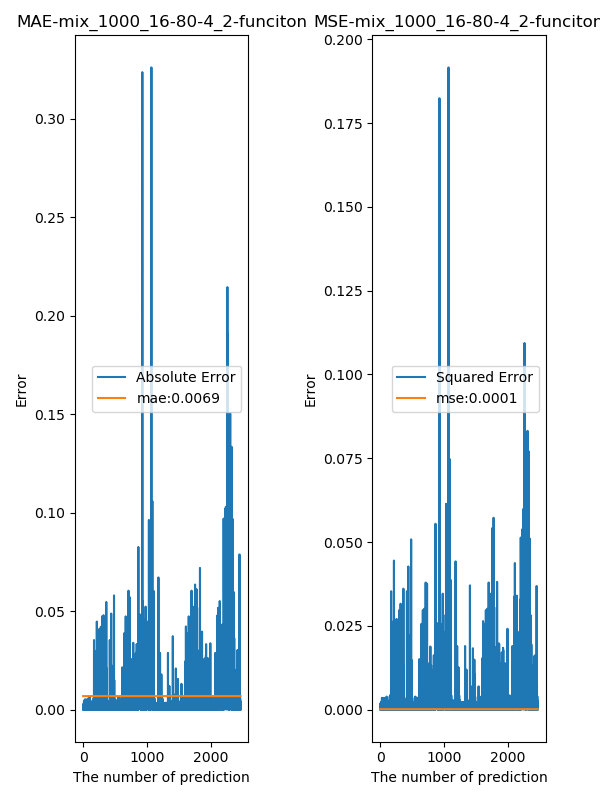
\includegraphics[scale=0.371]{png/result/mix_1000_16-80-4_2-funciton.png}
	\end{itemize}
\end{frame}


\begin{frame}
	\frametitle{\tiny 准确率:98.05\% ,微调总数据量:40000,四种不同序列和5种不同长度的组合,每种类型1000}
	\begin{itemize}
        \item 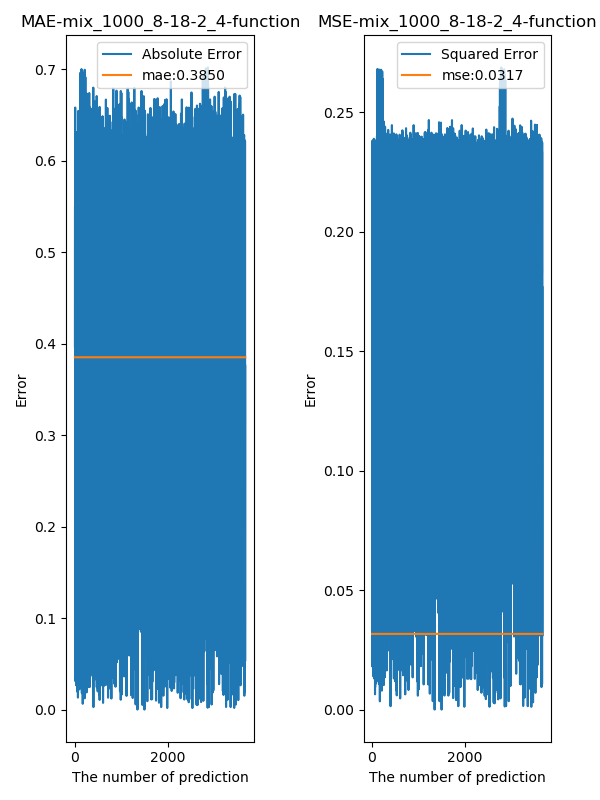
\includegraphics[scale=0.371]{png/result/mix_1000_8-18-2_4-function.png}
	\end{itemize}
\end{frame}

\begin{frame}
	\frametitle{\tiny 准确率:99.95\% ,微调总数据量:200000,4种不同序列和5种不同长度的组合,每种类型5000}
    % \frametitle{\tiny 微调总数据量:200000,四种不同序列和5种不同长度的组合,准确率:99.95\% }
	\begin{itemize}
        \item 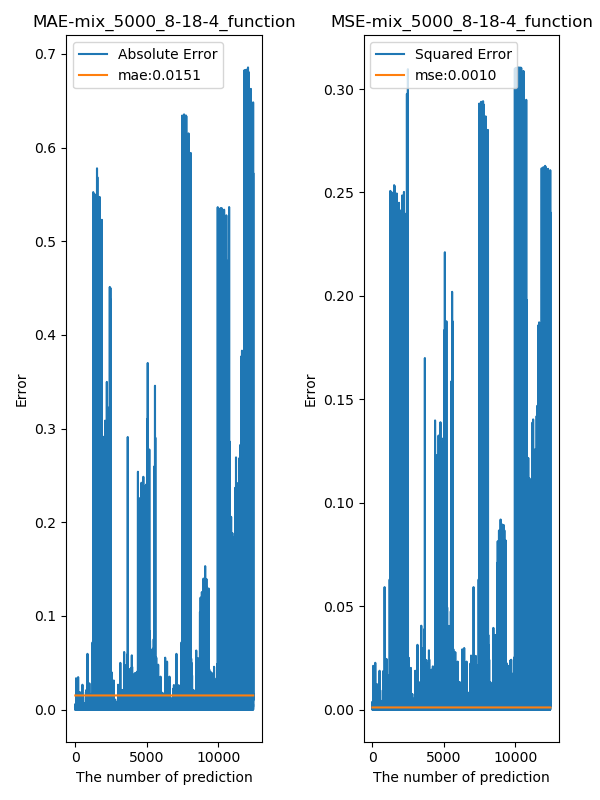
\includegraphics[scale=0.371]{png/result/mix_5000_8-18-4_function.png}
	\end{itemize}
\end{frame}

% \begin{frame}
% 	\frametitle{\small 总数据量:30000,16预测8,长向量序列预测}	
% 	\begin{itemize}
% 		% \item 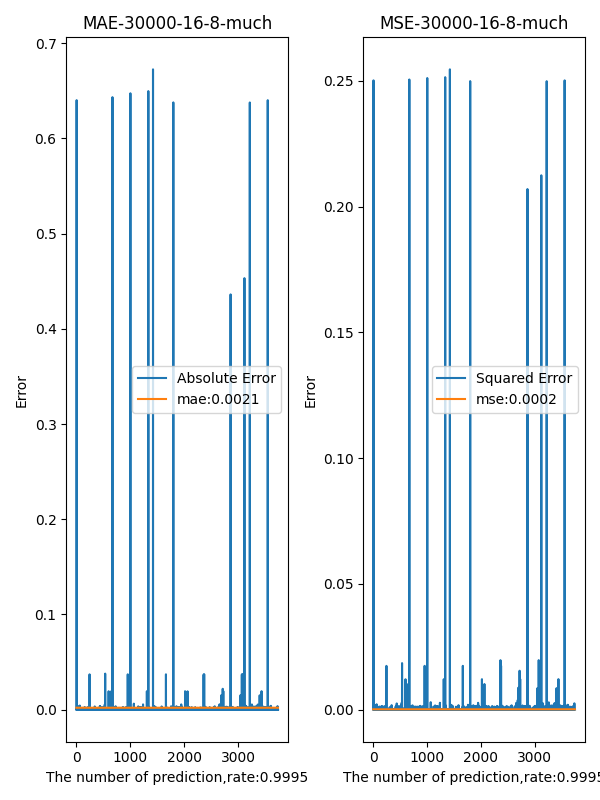
\includegraphics[scale=0.371]{png/30000-16-8-much.png}
% 	\end{itemize}
% \end{frame}

\subsection{实验结果分析}
\begin{frame}
	\frametitle{根据数据的结论}	
	\begin{itemize}
        \item 从中可以看出,不同的预测长度对于精确度影响不大,但是不同种的序列对精确度的影响比较大。
        \item 但类型数量取1000的时候,对于不同种类的序列会使得最终误差较大,但是提高数量到5000,能够让误差明显的变小。
		% \item 当预测任务,以及预测序列相同时,可以看出给定训练的序列越长,效果越好。
		% \item 当训练数据集的数量,测试的序列相同时,预测的长度越短,效果越好。
		% \item 当训练总数据集数量,预测长度相同时,训练的序列向量越长,对最终的预测结果更加精确。
		% \item 对于一个预测长度不一致的数据集合,最终的误差比较大,且预测序列长度和目标序列长度相似度大约是76\%
		% \item 从混合的预测长度,时间序列的数据集合训练结果中也可以看出这个长向量时间序列的预测结果要好于短向量的结果,且预测短的序列要优于预测长序列的误差。
	\end{itemize}
\end{frame}


% \subsection{实验过程中遇到的一些问题}

% \begin{frame}
% 	\frametitle{遇到的问题}	
% 	\begin{itemize}
%         \item 目标预测的个数和实际预测个数不同或者预测非数值形式,下面是一些解决方法
%         \eee{
%             \item 忽略实际预测个数和目标个数不同的例子,并计算其比率rate(目标与实际个数相同的个数/测试集个数)
%             \item 对预测得到的结果进行截断或补零
%         }   
%         \item 序列长度太长的问题
% 	\end{itemize}
%     % 目前考虑的是只考虑数量对等的
% \end{frame}


\subsection{下一步的计划}
\begin{frame}
	\frametitle{实现目标}	
	\begin{itemize}
        % \item 混合更多的元素,同时训练更多不同种类的时间序列和以及预测长度。
        \item 尝试对未见过的序列进行预测,看看结果如何。
        \item 修改提示方式,寻找更好的描述不同的特征的提示。
        \item 多种模型的测试,参考PromptCast论文中,不仅要有语言模型进行预测,还要用时间序列的模型预测来进行结果比对。
        \item 尝试使用其中一篇文章中的MEGABYTE方法来处理长序列进行建模,以解决时间数据集中序列过长的问题。
        % \item 对于结果多次试验,取平均
        % \item 提高模型参数精度,看看结果是否会有什么变化。        
        % \item 开始对8个常见的时间序列进行测试。
	\end{itemize}
\end{frame}

% \subsection{图像结果展示}
% \subsection{测试的数据集}


% \section{相关论文}
% \begin{frame}
%     \frametitle{prompt learning and time series论文(IEEE)}
% \eee{
%     \item 标题:Evaluating BERT on cloud-edge time series forecasting and sentiment analysis via prompt learning\\
%     \item 结论:该论文使用即时学习评估了在云边缘时间序列预测和情感分析任务的大量数据上预训练的BERT的性能。实验结果表明,BERT在云边时间序列预测任务中表现不佳,这表明BERT没有良好的逻辑推理能力。选择均方误差 (MSE) 作为时间序列预测的评估指标,结果表明,使用即时学习的 BERT 无法根据前一个滑动窗口中的信息很好地预测下一个时间步长的特征。
% }    
% \end{frame}


% 结束语
\section{}
\begin{frame}
	\frametitle{}
	\begin{center}
		\Huge{谢谢老师和同学的聆听!}
	\end{center}
\end{frame}

\end{CJK*}
\end{document}